\documentclass[book.tex]{subfiles}
\begin{document}
This chapter describes the target hardware of Wolfenstein 3D. For simplicity I chose to describe it as
a pipeline taking user commands as entries and outputting images and audio.

\begin{figure}[H]
\centering
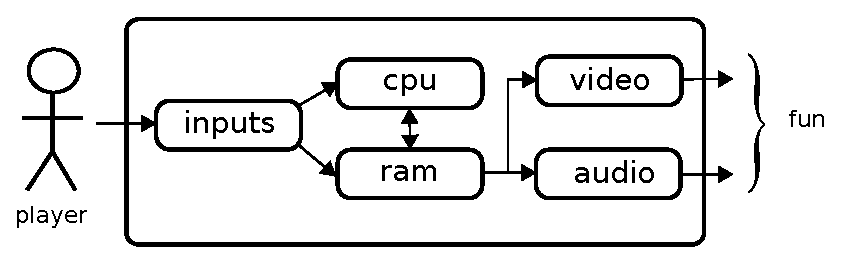
\includegraphics[scale=0.7]{imgs/fun_pipeline.eps}
%\def\svgscale{1.5}
%\input{imgs/fun_pipeline.pdf_tex}
\caption{Hardware pipeline.}
\label{fig:digraph}
\end{figure}

The pipeline is made of five parts, some of them were huge bottleneck for game development while others were unexpectedly
good:

\begin{figure}[H]
\centering
\begin{tabularx}{\textwidth}{ X X  }
  \toprule
  \textbf{Stage} & \textbf{Quality} \\ \bottomrule
  CPU & Poor \\ 
  RAM & Very Poor \\ 
  Video & Poor \\ 
  Audio & Good \\ 
  Inputs & Good \\ \bottomrule
\end{tabularx}
\label{fig:Pipeline stages}
\end{figure}

Overall, the pipeline offered a lot of friction: hardware manufacturers had not embraced the game industry yet. Personal computers were designed to display static images and crunch integers. Real-time 3D, fractions and smooth 60 fps animations were not part of the blueprints.

\section{CPU}
  \subsection{History}
  The ubiquitous CPU manufacturer was Intel with its x86 line of microprocessors.  The i286 machines released in 1982 were declining and replaced by Intel's first 32 bits processor: The i386. Moore's law was in full effect and the high end i386-DX 33Mhz was a beast. The power increase is obvious when plotted on a MIPs\footnote{Million Instructions Per Second.} histogram:


\definecolor{skyblue1}{rgb}{0.1,0.624,0.812}


\begin{figure}[H]
\centering
  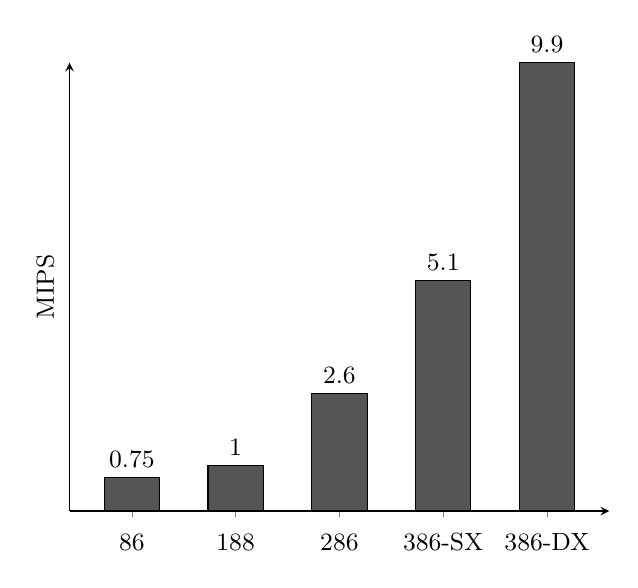
\begin{tikzpicture}[font=\small]
    \begin{axis}[
      ybar,
      bar width=20pt,
      ylabel={MIPS},
      ymin=0,
      ytick=\empty,
      xtick=data,
      axis x line=bottom,
      axis y line=left,
      enlarge x limits=0.15,
      symbolic x coords={86,188,286,386-SX,386-DX},
      xticklabel style={anchor=base,yshift=-\baselineskip},
      nodes near coords={\pgfmathprintnumber\pgfplotspointmeta}
    ]
      \addplot[fill={rgb:red,0.5;green,0.5;blue,0.5}] coordinates {
        (86,0.75)
        (188,1)
        (286,2.6)
        (386-SX,5.1)
        (386-DX,9.9)
      };
    \end{axis}
    
   \end{tikzpicture}
   \caption{Processor speeds comparaison.} \label{fig:mips}
 \end{figure}

 \textbf{\underline{Trivia :}} To keep things into perspective, a modern processor such as the Intel Core i7 3.33 GHz operates at close to 180,000 Mips: Five orders of magnitude faster!

 \bigskip

\textbf{\underline{Trivia :}}  Two other companies were producing 386 clones: AMD and Cyrix. The mediocre performances did not justify the lower cost and as a result they never gathered a significant market share. Interestingly AMD evolved to become a serious challenger while Cyrix merged with National Semiconductor in 1997.
  \subsection{Floating Point}
  
  Since the 286 systems were progressively being replaced with 386, it was decided Wolfenstein 3D target machine would be a low-end 386 machine (while still being playable on a 286 with reduced view). 
  \bigskip

  In order to perform all the trigonometric operations, the C language offered the types \emph{float} and \emph{double} which kept track of the fractional part of each operations.


  

  Unfortunately if Intel CPUs were good at crunching integers, they were not good at all for the calculations necessary in a 3D game: Trigonometric functions need to keep track of fractions. Developers could use C language's  when writing software but the problem came from the hardware:\bigskip

  CPUs had no floating point unit.
   \bigskip
   As a result, those operations were emulated by the compiler and therefore impossibly slow. At first sight it looked like fractions and 3D were out of the picture. A workaround had to be found.


    slow: higher precision
          same window
          all registers were 16 bits.
\bigskip


  
     Floating point are god sent format to 3D programmers.

  \subsection{Fixed Point}
  Integers were not accurate enough and floating point too slow. How could one perform operation while preserving the fractional part of a number ? The answer was to re-purpose the hardware via Fixed Point arithmetic.
\begin{figure}[H]
\centering
 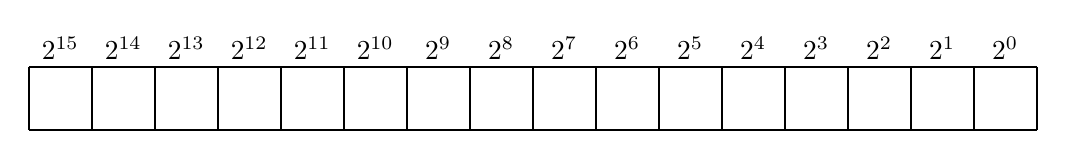
\begin{tikzpicture}[scale=0.8, every node/.style={scale=0.99}]
\draw[thick] (0,0) -- (16,0);
\draw[thick] (0,1) -- (16,1);
\foreach \i in {0,...,16}
{
     \draw[thick] (\i,1) -- (\i,0);
}

\foreach \i in {0,...,15}
{
     \node[] at (15-\i+0.5,1.3){$2^{\i}$}  ;
       
       
     
}
\end{tikzpicture}

 \caption{Integer layout.} \label{fig:mips}
 \end{figure}

\begin{figure}[H]
\centering
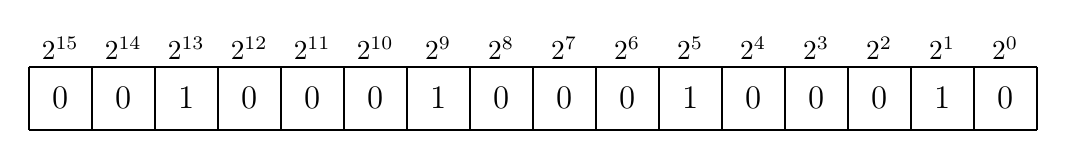
\begin{tikzpicture}[scale=0.8, every node/.style={scale=0.99}]
\draw[thick] (0,0) -- (16,0);
\draw[thick] (0,1) -- (16,1);
\foreach \i in {0,...,16}
{
     \draw[thick] (\i,1) -- (\i,0);
}

\foreach \i in {0,...,15}
{
     \node[] at (15-\i+0.5,1.3){$2^{\i}$}  ;
}

\tikzstyle{fontbf} = [font=\large]
\node[fontbf] at (0.5,0.5){0} ;
\node[fontbf] at (1.5,0.5){0};  
\node[fontbf] at (2.5,0.5){1} ; 
\node[fontbf] at (3.5,0.5){0} ;

\node[fontbf] at (4.5,0.5){0} ;
\node[fontbf] at (5.5,0.5){0};  
\node[fontbf] at (6.5,0.5){1} ; 
\node[fontbf] at (7.5,0.5){0} ;

\node[fontbf] at (8.5,0.5){0} ;
\node[fontbf] at (9.5,0.5){0};  
\node[fontbf] at (10.5,0.5){1} ; 
\node[fontbf] at (11.5,0.5){0} ;

\node[fontbf] at (12.5,0.5){0} ;
\node[fontbf] at (13.5,0.5){0};  
\node[fontbf] at (14.5,0.5){1} ; 
\node[fontbf] at (15.5,0.5){0} ;


\end{tikzpicture}

 \caption{Integer example.} \label{fig:mips}
 \end{figure}

\begin{figure}[H]
 \centering
  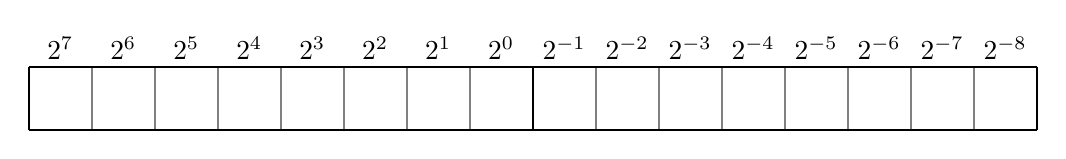
\begin{tikzpicture}[scale=0.8, every node/.style={scale=0.99}]


\colorlet{LighterMark}{black!50}

\foreach \i in {1,...,15}
{
     \draw[thick,LighterMark] (\i,1) -- (\i,0);
}

     \draw[thick,black] (0,1) -- (0,0);
      \draw[thick,black] (8,1) -- (8,0);
      \draw[thick,black] (16,1) -- (16,0);
      
\draw[thick,black] (0,0) -- (16,0);
\draw[thick,black] (0,1) -- (16,1);
 

%\foreach \i[evaluate={\pow=int(7-\i)}] in {0,...,7}
\foreach \i[evaluate={\pow=int(7-\i)}] in {0,...,7}
{
   \node[] at (\i+0.5,1.3){$2^{\pow}$  }  ;
      
         
     
}

%\foreach \i[evaluate={\pow=int((\i-7)*2)}]  in {8,...,15}
\foreach \i[evaluate={\pow=int(\i-7)}]  in {8,...,15}
{
     \node[] at (\i+0.5,1.3){$2^{-\pow}$}  ;
}




\end{tikzpicture}

 \caption{Fixed point layout.} \label{fig:mips}
\end{figure}

\begin{figure}[H]
 \centering
   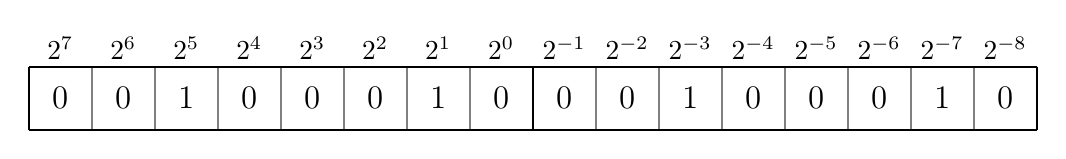
\begin{tikzpicture}[scale=0.8, every node/.style={scale=0.99}]


\colorlet{LighterMark}{black!50}

\foreach \i in {1,...,15}
{
     \draw[thick,LighterMark] (\i,1) -- (\i,0);
}

     \draw[thick,black] (0,1) -- (0,0);
      \draw[thick,black] (8,1) -- (8,0);
      \draw[thick,black] (16,1) -- (16,0);
      
\draw[thick,black] (0,0) -- (16,0);
\draw[thick,black] (0,1) -- (16,1);
 

%\foreach \i[evaluate={\pow=int(7-\i)}] in {0,...,7}
\foreach \i[evaluate={\pow=int(7-\i)}] in {0,...,7}
{
   \node[] at (\i+0.5,1.3){$2^{\pow}$  }  ;
      
         
     
}

%\foreach \i[evaluate={\pow=int((\i-7)*2)}]  in {8,...,15}
\foreach \i[evaluate={\pow=int(\i-7)}]  in {8,...,15}
{
     \node[] at (\i+0.5,1.3){$2^{-\pow}$}  ;
}

\tikzstyle{fontbf} = [font=\large]
\node[fontbf] at (0.5,0.5){0} ;
\node[fontbf] at (1.5,0.5){0};  
\node[fontbf] at (2.5,0.5){1} ; 
\node[fontbf] at (3.5,0.5){0} ;

\node[fontbf] at (4.5,0.5){0} ;
\node[fontbf] at (5.5,0.5){0};  
\node[fontbf] at (6.5,0.5){1} ; 
\node[fontbf] at (7.5,0.5){0} ;

\node[fontbf] at (8.5,0.5){0} ;
\node[fontbf] at (9.5,0.5){0};  
\node[fontbf] at (10.5,0.5){1} ; 
\node[fontbf] at (11.5,0.5){0} ;

\node[fontbf] at (12.5,0.5){0} ;
\node[fontbf] at (13.5,0.5){0};  
\node[fontbf] at (14.5,0.5){1} ; 
\node[fontbf] at (15.5,0.5){0} ;


\end{tikzpicture}

  \caption{Fixed point example.} \label{fig:mips}
\end{figure} 

 \textbf{\underline{Trivia :}} Fixed Point has its own notation called “Q”. A Q1.14 number has 1 integer bit and 14 fractional bits.

\bigskip

 \textbf{\underline{Trivia :}}  Fixed Point Arithmetic usage was not limited to PC gaming. Many game console manufactured later still had no hardware floating point unit: Sony's original PlayStation (1994) and Sega's Saturn (1994) are few examples among many with a design choice that not only reduced the production cost but also maximized the CPU pipeline throughput. 

\bigskip

\section{RAM}
  386 very powerful (run Linux 4GB, MMU) buy a major obstacle stood between the programmer and the machine. It was the operating system and its name was DOS 4.0.
  \bigskip
  \subsection{DOS limitations}

  \subsection{16 bits Segmented RAM}

\begin{verbatim}
    0110 1000 1000 0111 0000  Segment, 16 bits shifted 4 bits left  
  +      0011 0100 1010 1001  Offet,   16 bits
============================
    0110 1011 1101 0001 1001  Address, 20 bits
\end{verbatim}

  \subsection{Extended Memory}
  
\section{Video}
  \subsection{VGA Architecture}
  \subsection{VGA setup}
  \subsection{VGA Programming}
  \subsection{VGA Mode Y}
\section{Audio}
  \subsection{Speaker}
  \subsection{Ad Lib}
  \subsection{Sound Blaster}

\section{Inputs}

\end{document}




